\documentclass[12pt]{article}

\usepackage[margin=1in]{geometry}
\usepackage{amsmath,amsthm,amssymb}
\usepackage{float}
\usepackage{graphicx}
\usepackage{bbold}
\usepackage{algorithm}
\usepackage{algcompatible}
\usepackage{csquotes}
\usepackage{url}
\usepackage{enumerate}

\newcommand{\N}{\mathbb{N}}
\newcommand{\Z}{\mathbb{Z}}
\newcommand{\abs}[1]{\left| #1 \right|}
\newcommand{\norm}[1]{\left|\left| #1 \right|\right|}
\newcommand{\ceil}[1]{\left\lceil #1 \right\rceil}
\newcommand{\floor}[1]{\left\lfloor #1 \right\rfloor}
\newcommand{\pprime}{\prime \prime}
\newcommand{\BigO}[1]{\mathcal{O}\left( #1 \right)}
\newcommand{\proj}[2][]{\textit{proj}_{\vect{#1}}\vect{#2}}
\newcommand{\vect}{\mathbf}
\newcommand{\Id}{\mathbb{1}}
\newcommand{\inv}[1]{ #1^{-1}}
\newcommand{\minn}{\text{min}}
\newcommand{\maxx}{\text{max}}
\renewcommand{\P}[1]{\left( #1 \right)}
\newcommand{\diag}[1]{\text{diag}\P{#1}}
\newcommand{\grad}{\nabla}
\newcommand{\laplacian}{\nabla^{2}}

\newenvironment{theorem}[2][Theorem]{\begin{trivlist}
\item[\hskip \labelsep {\bfseries #1}\hskip \labelsep {\bfseries #2.}]}{\end{trivlist}}
\newenvironment{lemma}[2][Lemma]{\begin{trivlist}
\item[\hskip \labelsep {\bfseries #1}\hskip \labelsep {\bfseries #2.}]}{\end{trivlist}}
\newenvironment{exercise}[2][Exercise]{\begin{trivlist}
\item[\hskip \labelsep {\bfseries #1}\hskip \labelsep {\bfseries #2.}]}{\end{trivlist}}
\newenvironment{problem}[2][Problem]{\begin{trivlist}
\item[\hskip \labelsep {\bfseries #1}\hskip \labelsep {\bfseries #2.}]}{\end{trivlist}}
\newenvironment{question}[2][Question]{\begin{trivlist}
\item[\hskip \labelsep {\bfseries #1}\hskip \labelsep {\bfseries #2.}]}{\end{trivlist}}
\newenvironment{corollary}[2][Corollary]{\begin{trivlist}
\item[\hskip \labelsep {\bfseries #1}\hskip \labelsep {\bfseries #2.}]}{\end{trivlist}}

\renewcommand{\algorithmicrequire}{\textbf{Input:}}
\renewcommand{\algorithmicensure}{\textbf{Output:}}

\DeclareMathOperator{\sech}{sech}
\DeclareMathOperator{\csch}{csch}

\begin{document}

\title{CS6210: Homework 6}
\author{Christopher Mertin}
\date{December 8, 2016}
\maketitle

\begin{enumerate}
%%%%%% Problem 1 %%%%%%
\item 

\begin{enumerate}
\item Using an orthogonal polynomial basis, find the best least squares polynomial approximations, $q_{2}(t)$ of degree at most 2 and $q_{3}(t)$ of degree at most 3, to $f(t) = e^{-3t}$ over the interval $[0,3]$.

[Hint: For a polynomial $p(x)$ of degree $n$ and a scalar $a > 0$ we have $\int e^{-ax}p(x)\text{d}x = -\frac{e^{-ax}}{a}\ \left( \sum_{j=0}^{n} \frac{p^{(j)}(x)}{a^{j}}\right)$, where $p^{(j)}(x)$ is the $j^{th}$ derivative of $p(x)$. Alternatively, just use numerical quadrature, e.g., the {\sc Matlab} function {\tt quad}.]

{\bf Solution:}

In the general case, we can use Legendre Polynomials. Were first we can find $x$ with respect to $t$ as being

\begin{align*}
x &= \frac{2t-a-b}{b-a} = \frac{2t-0-3}{3-0} = \frac{2t-3}{3} = \frac{2}{3}t - 1\\
\intertext{Giving us our parameters to be}
\phi_{0} &= 1\\
\phi_{1} &= x = \frac{2}{3}t - 1\\
\phi_{2} &= \frac{1}{2}\left( 3x^{2} - 1\right) = \frac{1}{2}\left( 3 \left(\frac{2}{3}t - 1\right)^{2}-1\right) = \frac{2}{3}t^{2} - 2t + 1\\
\phi_{3} &= \frac{1}{27}\left( 20t^{3} - 90t^{2} + 114t - 36\right)\\
c_{0} &= \frac{\int_{0}^{3}e^{-3t}\text{d}t}{\int_{0}^{3}\text{d}t} = \frac{1 - e^{-9}}{9}\\
c_{1} &= \frac{\int_{0}^{3}\left( \frac{2}{3}t - 1\right) e^{-3t}\text{d}t}{\int_{0}^{3}\left( \frac{2}{3}t - 1\right)^{2}\text{d}t} = \frac{-7 -11e^{-9}}{27}\\
c_{2} &= \frac{\int_{0}^{3}\left( \frac{2}{3}t^{2} - 2t + 1\right)e^{-3t}\text{d}t}{\int_{0}^{3}\left( \frac{2}{3}t^{2} - 2t + 1 \right)^{2}\text{d}t} = \frac{65 - 245 e^{-9}}{243}\\
c_{3} &= \frac{\int_{0}^{3}\left( \frac{1}{27}\left( 20t^{3} - 90t^{2} + 114t - 36\right)\right)e^{-3t}\text{d}t}{\int_{0}^{3}\left( \frac{1}{27}\left( 20t^{3} - 90t^{2} + 114t - 36\right)\right)^{2}\text{d}t} = \frac{-413 - 5299e^{-9}}{2187}
\end{align*}

We can then put $\phi_{i}$ and $c_{i}$ into our approximation of the formua:

\[
v(x) = \sum_{j=0}^{n}c_{j}\phi_{j}(x)
\]

By using $n = 2$ we get $q_{2}(x)$ and by using $n = 3$ we get $q_{3}(x)$.

\item Plot the error functions $f(t) - q_{2}(t)$ and $f(t) - q_{3}(t)$ on the same graph on the interval $[0,3]$. Compare the errors of the two approximating polynomials. In the least squares sense, which polynomial provides the better approximation?

[Hint: In each case you may compute the {\em norm} of the error, $\left( \int_{a}^{b}(f(t) - q_{n}(t))^{2}\text{d}t \right)^{2}$, using the {\sc Matlab} function {\tt quad}]

{\bf Solution:}

\begin{figure}[H]
\centering
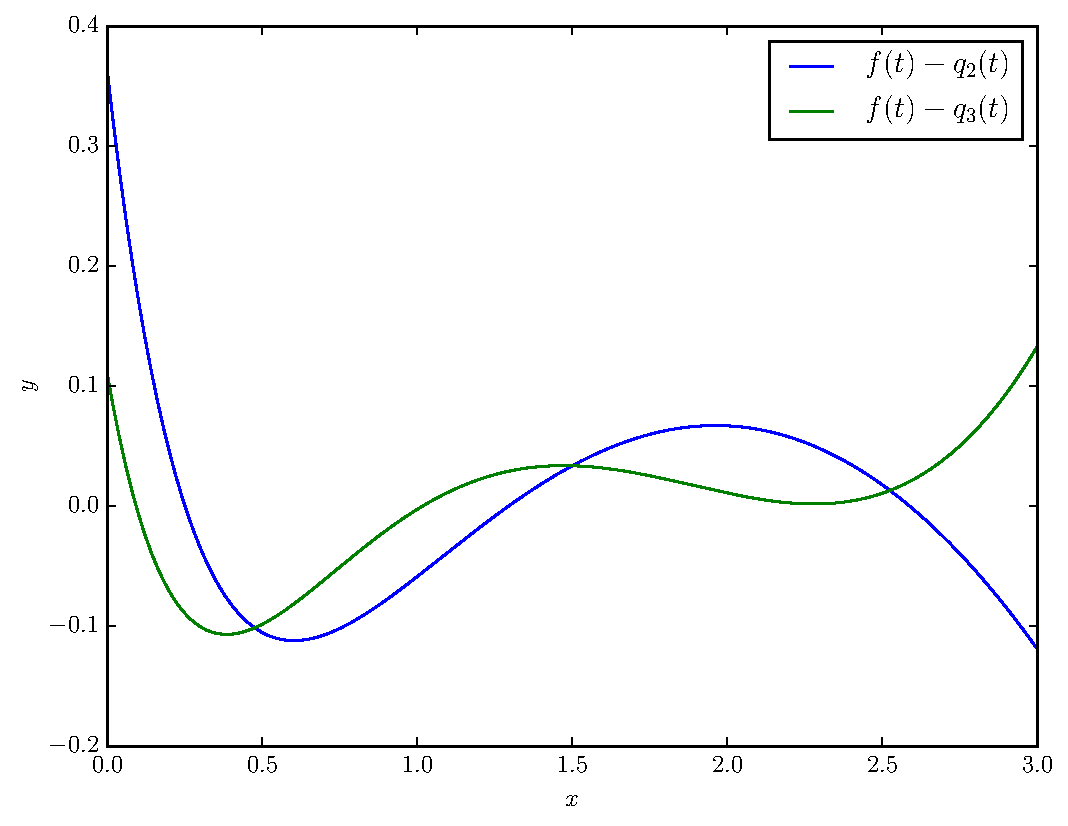
\includegraphics[width=.75\textwidth]{plot1.pdf}
\caption{See {\tt prob1.py}}
\end{figure}

\item Without any computation, prove that $q_{3}(t)$ generally provides a least squares fit, which is never worse than with $q_{2}(t)$. 

{\bf Solution:}

In general, for lower power polynomial expressions the higher polynomial that is used, the more accurate the result. Therefore $q_{3}(t)$ would provide the better approximation since it is $n = 3$ compared to $n = 2$ for $q_{2}(x)$, and the powers are not high enough to produce high oscillations. 
\end{enumerate}

\newpage

\item Let $f(x)$ be a given function that can be evaluated at points $x_{0} \pm jh,\ j=\{0,1,2,\ldots\}$ for any fixed value of $h$, $0 < h \ll 1$.

\begin{enumerate}
\item Find a second order formula (i.e., trunctation error $\BigO{h^{2}}$) approximating the third derivative $f^{\prime \prime \prime}(x_{0})$. Give the formula, as well as an expression for the truncation error, i.e. not just its order

{\bf Solution:}

We can use the following four equations:

\begin{align*}
f(x_{0}+h) &= f(x_{0}) + hf^{\prime}(x_{0}) + \frac{h^{2}}{2}f^{\pprime}(x_0) + \frac{h^{3}}{6}f^{(3)}(x_{0}) + \frac{h^{4}}{24}f^{(4)}(x_{0}) + \frac{h^{5}}{120}f^{(5)}(\xi_{1})\\
f(x_{0}-h) &= f(x_{0}) - hf^{\prime}(x_{0}) + \frac{h^{2}}{2}f^{\pprime}(x_0) - \frac{h^{3}}{6}f^{(3)}(x_{0}) + \frac{h^{4}}{24}f^{(4)}(x_{0}) - \frac{h^{5}}{120}f^{(5)}(\xi_{1})\\
f(x_{0}+2h) &= f(x_{0}) + 2hf^{\prime}(x_{0}) + 2h^{2}f^{\pprime}(x_0) + \frac{8h^{3}}{6}f^{(3)}(x_{0}) + \frac{16h^{4}}{24}f^{(4)}(x_{0}) + \frac{32h^{5}}{120}f^{(5)}(\xi_{1})\\
f(x_{0}-2h) &= f(x_{0}) - 2hf^{\prime}(x_{0}) + 2h^{2}f^{\pprime}(x_0) - \frac{8h^{3}}{6}f^{(3)}(x_{0}) + \frac{16h^{4}}{24}f^{(4)}(x_{0}) - \frac{32h^{5}}{120}f^{(5)}(\xi_{1})\\
\end{align*}

After subtracting the first two equations and using the intermediate value theorem:

\begin{align*}
f(x_{0} + h) - f(x_{0} - h) &= 2hf^{\prime}(x_{0}) + \frac{h^{3}}{3}f^{(3)}(x_{0}) + \frac{h^{5}}{60}f^{(5)}(\eta_{1})
\end{align*}

Finding $f^{\prime}(x_{0})$

\begin{align*}
2hf^{\prime}(x_{0}) &= f(x_{0} + h) - f(x_{0} - h) - \frac{h^{3}}{3}f^{(3)}(x_{0}) - \frac{h^{5}}{60}f^{(5)}(\eta_{1})\\
f^{\prime}(x_{0}) &= \frac{1}{2h}\left( f(x_{0} + h) - f(x_{0} - h) - \frac{h^{3}}{3}f^{(3)}(x_{0}) - \frac{h^{5}}{60}f^{(5)}(\eta_{1})\right)\\
\intertext{After subtracting the second two equations and using the intermediate value theorem for the error terms:}
f(x_{0} + 2h) -& f(x_{0} - 2h) = 4hf^{\prime}(x_{0}) + \frac{8h^{3}}{3}f^{(3)}(x_{0}) + \frac{32h^{5}}{60}f^{(5)}(\eta_{2})\\
\intertext{Finding $f^{\prime}(x_{0})$:}
4hf^{\prime}(x_{0}) &= f(x_{0} + 2h) - f(x_{0} - 2h) - \frac{8h^{3}}{3}f^{(3)}(x_{0}) - \frac{32h^{5}}{60}f^{(5)}(\eta_{2})\\
f^{\prime}(x_{0}) &= \frac{1}{4h}\left( f(x_{0} + 2h) - f(x_{0} - 2h) - \frac{8h^{3}}{3}f^{(3)}(x_{0}) - \frac{32h^{5}}{60}f^{(5)}(\eta_{2})\right)
\end{align*}

After subtracting these two equations for $f^{\prime}(x_{0})$ and solving for $f^{(3)}(x_{0})$, we have

\begin{align*}
\frac{6h^{3}}{2}f^{(3)}(x_{0}) &= \frac{1}{4h}\left( f(x_{0} + 2h) - f(x_{0} - 2h) + 2f(x_{0} - h) - 2f(x_{0} + h) - \frac{1}{2}h^{5}f^{(5)}(\eta)\right)\\
f^{(3)}(x_{0}) &=\frac{1}{8h^{3}}\left( f(x_{0} + 2h) - f(x_{0} - 2h) + 2f(x_{0} - h) - 2f(x_{0} + h) - \frac{1}{2}h^{5}f^{(5)}(\eta)\right)
\end{align*}

We used the intermediate value theorem to find $\eta$. 

\item Use your formula to provide approximations to $f^{(3)}(0)$ for the function $f(x) = e^{x}$ employing values $h = \{ 10^{-1}, 10^{-2}, \ldots, 10^{-9}\}$, with the default ${\tt Matlab}$ arithmetic. Verify that for the larger values of $h$ your formula is indeed second order accurate. Which value of $h$ gives the closest approximation to $e^{0} = 1$?

{\bf Solution:}


\begin{table}[H]
\centering
\begin{tabular}{l r}
\hline \hline
$h$ & $f^{(3)}(x_{0})$\\
\hline
0.1 & 2.5063e-07\\
0.01 & 2.5001e-13\\
0.001 & 2.5000e-19\\
0.0001 & 2.5002e-25\\
1e-05 & 2.7756e-31\\
1e-06 & 0.0000e+00\\
1e-07 & 5.5511e-38\\
1e-08 & 0.0000e+00\\
1e-09 & 0.0000e+00\\
\hline
\end{tabular}
\caption{See {\tt prob2.py}}
\end{table}

Which shows that the formula is indeed $2^{nd}$ order accurate. The best value of $h$ that would be the most accurate is the largest, $h = 0.1$, which produces a value that is closest to the true value.

\item For the formual that you derived in (a), how does the roundoff error behave as a function of $h$, as $h\rightarrow 0$.

{\bf Solution:}

$\widetilde{f}(x)$ is the approximation for $f(x)$:

\begin{align*}
\widetilde{f}(x) = f(x) + e_{r}(x)\\
\intertext{We do the same calculations on page 422}
\abs{f^{\prime}(x_{0}) - \widetilde{D}} &= \abs{ (f^{\prime}(x_{0}) - D) + (D - \widetilde{D})} \leq \abs{ f^{\prime}(x_{0}) - D} + \abs{D - \widetilde{D}}\\
\intertext{As we calculated in part a}
\abs{f^{\prime}(x_{0}) - D} &= \frac{1}{16}h^{2}f^{(5)}(\eta)\\
\intertext{And if $M$ is a maximum for $f^{(5)}(x)$ on its whole domain, then}
\abs{f^{\prime}(x_{0}) - D} &\leq \frac{1}{16}h^{2}M\\
\intertext{As an upper bound for $\abs{D - \widetilde{D}}$ we have $6\epsilon/h^{3}$ because: two $\epsilon$ for points $x_{0} + h$ and $x_{0} - h$ and two $2\epsilon$ for $x_{0} + 2h$ and $x_{0} - 2h$}
\abs{D - \widetilde{D}} &= \frac{6\epsilon}{h^{3}}\\
\end{align*}

Putting these two together

\[
\abs{f^{\prime}(x_{0}) - \widetilde{D}} = \abs{(f^{\prime}(x_{0}) - D) + (D - \widetilde{D})} \leq \abs{f^{\prime}(x_{0}) - D} + \abs{D - \widetilde{D}} \leq \frac{1}{16}h^{2}M + \frac{6\epsilon}{h^{3}}
\]

as $h\rightarrow 0$, the function blows up since there is a cubic $h$ in the denominator but a square term in the numerator.

\item How would you go about obtaining a forth order formula for $f^{(3)}(x_{0})$ in general? (You don't have to actually derive it: just describe in one or two sentences.) How many points would this formula require?

{\bf Solution:}

We can use seven points: $x_{0}$, $x_{0} + h$, $x_{0} - h$, $x_{0} + 2h$, $x_{0} - 2h$, $x_{0} + 3h$, $x_{0} - 3h$, and do similar computations for the fourth order as we did above.
\end{enumerate}

\newpage

\item Consider the derivation of an approximate formula for the second derivative $f^{\prime \prime}(x_{0})$ of a smooth function $f(x)$ using three points $x_{-1},\ x_{0}=x_{-1} + h_{0},\ \text{and}\ x_{1}=x_{0}+h_{1}$, where $h_{0} \neq h_{1}$. 

Consider the following two methods:

\begin{enumerate}[i.]
\item Define $g(x) = f^{\prime}(x)$ and seek a {\em staggered mesh}, centered approximiations as follows:

\begin{align*}
g_{1/2} &= \frac{f(x_{1}) - f(x_{0})}{h_{1}};\quad g_{-1/2} = \frac{f(x_{0}) - f(x_{-1})}{h_{0}}\\
f^{\prime \prime}(x_{0}) &\approx \frac{g_{1/2} - g_{-1/2}}{(h_{0} + h_{1})/2}
\end{align*}

The idea is that all of the differences are short(i.e., not long differences) and centered.

\item Using the second degree interpolating polynomial in Newton form, differentiated twice, define

\[
f^{\prime \prime}(x_{0}) \approx 2f[x_{-1}, x_{0}, x_{1}]
\]

\end{enumerate}

Here is where you come in:

\begin{enumerate}
\item Show that the above two methods are one in the same

{\bf Solution:}

\begin{align*}
f^{\pprime}(x_{0}) &= \frac{g_{1/2} - g_{-1/2}}{(h_{0} + h_{1})/2} = \frac{\frac{f(x_{1}) - f(x_{0})}{x_{1} - x_{0}} - \frac{f(x_{0}) - f(x_{-1})}{x_{0} - x_{-1}}}{\frac{x_{1} - x_{-1}}{2}}\\
&= \frac{\frac{f(x_{1}) - f(x_{0})}{x_{1} - x_{0}} - \frac{f(x_{0}) - f(x_{-1})}{x_{0} - x_{-1}}}{x_{1} - x_{-1}} = 2f[x_{-1}, x_{0}, x_{1}]
\end{align*}

\item Show that this method is only first order accurate in general

{\bf Solution:}

We can use the Taylor expansion of $f$ around $x_{1}$:

\begin{align*}
f(x_{1}) &= f(x_{0} + h_{1}) = f(x_{0}) + h_{1}f^{\prime}(x_{0}) + \frac{h_{1}^{2}}{2}f^{\pprime}(x_{0}) + \frac{h_{1}^{3}}{3!}f^{(3)}(\eta_{1})\\
\intertext{Now we can rewrite $g_{1/2}$ as}
g_{1/2} &= \frac{f(x_{1}) - f(x_{0})}{h_{1}} = f^{\prime}(x_{0}) + \frac{h_{1}}{2}f^{\pprime}(x_{0}) + \frac{h_{1}^{2}}{3!}f^{(3)}(\eta_{1})
\end{align*}

We can use the Taylor expansion of $f$ around $x_{0}$:

\begin{align*}
f(x_{0}) &= f(x_{-1} + h_{0}) = f(x_{-1}) + h_{0}f^{\prime}(x_{-1}) + \frac{h_{0}^{2}}{2}f^{\pprime}(x_{-1}) + \frac{h_{0}^{3}}{3!}f^{(3)}(\eta_{2})\\
\intertext{Now we can rewrite $g_{-1/2}$ as}
g_{-1/2} &= \frac{f(x_{0}) - f(x_{-1})}{h_{0}} = f^{\prime}(x_{-1}) + \frac{h_{0}}{2}f^{\pprime}(x_{-1}) + \frac{h_{0}^{2}}{3!}f^{(3)}(\eta_{2})
\end{align*}

To prove that $f^{\pprime}(x_{0})$ is first order accurate we just need to consider the last expression in $g_{1/2}$ and $g_{-1/2}$ in the formula $f^{\pprime}(x_{0})$. The formula for $f^{\pprime}(x_{0})$ is:

\[
f^{\pprime}(x_{0}) = \frac{g_{1/2} - g_{-1/2}}{(h_{0} + h_{1})/2}
\]

So we just consider the last expression in $g_{1/2}$ and $g_{-1/2}$:

\[
f^{\pprime}(x_{0}) = 2\frac{\frac{h_{1}^{2}}{3!}f^{(3)}(\eta_{1}) - \frac{h_{0}^{2}}{3!}f^{(3)}(\eta_{2})}{h_{0} + h_{1}}
\]

we find $\eta$ by using the intermediate value theorem:

\begin{align*}
f^{\pprime} &=  2\frac{\frac{h_{1}^{2}}{3!}f^{(3)}(\eta_{1}) - \frac{h_{0}^{2}}{3!}f^{(3)}(\eta_{2})}{h_{0} + h_{1}}\\
                    &= 2 \frac{\left(\frac{h_{1}^{2}}{3!} - \frac{h_{0}^{2}}{3!}\right)f^{(3)}(\eta)}{h_{0} + h_{1}}
\end{align*}

The numerator is of $\BigO{h^{2}}$ while the denominator is $\BigO{h}$, so it's overall $\BigO{h}$.

\item Run the two methods for the example depicted in Table 14.2 (but for the second derivative of $f(x) = e^{x}$). Report your findings.

{\bf Solution:}


\begin{table}[H]
\centering
\begin{tabular}{l c r}
\hline\hline
$h$ & $e_{n}$ & $e_{m}$\\
\hline
0.1  &  1.7302e-02  &  1.7302e-02 \\
0.01  &  1.6729e-03  &  1.6729e-03 \\
0.001  &  1.6673e-04  &  1.6673e-04 \\
0.0001  &  1.6662e-05  &  1.6662e-05 \\
0.00001  &  8.2742e-08  &  8.2755e-08 \\
\hline
\end{tabular}
\caption{See {\tt prob3.py}}
\end{table}

Where $e_{n}$ stands for the newton method and $e_{m}$ is for the mesh. What these results show is that both of the methods are linear in $h$ and both agree in value {\em until} they get down to $10^{-5}$, at which point they start to vary, but not a lot. This variance is most likely due to numerical error/truncation. Both methods are $\BigO{h}$ which agrees with our derivations above.



\end{enumerate}

\item Continuing with the notation of Exercise 12 (page 437), one could define 

\[
	g_{1/2} = \frac{f_{1} - f_{0}}{h}\quad \text{and}\quad g_{-1/2}=\frac{f_{0} - f_{-1}}{h}
\]

These approximate to second order the first derivative values $f^{\prime}(x_{0} + h/2)$ and $f^{\prime}(x_{0} - h/2)$, respectively. Then define

\[
	f_{pp_{0}} = \frac{g_{1/2} - g_{-1/2}}{h}
\]

All three derivative approximations here are centered (hence second order), and they are applied to first derivatives and hence have roundoff error increeasing proportionally to $h^{-1}$, not $h^{-2}$. Can we manage to (partially) cheat the hangman way?!

\begin{enumerate}
\item Show that in exact arithmetic $f_{pp_{0}}$ defined above and in Exercise 12 are one in the same

{\bf Solution:}

\begin{align*}
f_{pp_{0}} &= \frac{g_{1/2} - g_{-1/2}}{h} = \frac{\frac{f_{1} - f_{0}}{h} - \frac{f_{0} - f_{-1}}{h}}{h}\\
             &= \frac{f_{1} - f_{0} - f_{0} + f_{-1}}{h^{2}}
\end{align*}

Which is equal to the expression in Exercise 12.

\item Implement this method and compare to the results of Exercise 12. Explain your observations

{\bf Solution:}

\begin{table}[H]
\centering
\begin{tabular}{l r}
\hline \hline
$h$ & $f_{pp_{0}}$\\
\hline
$10^{-0.0}$  &  -0.85691 \\
$10^{-0.5}$  &  -0.92430 \\
$10^{-1.0}$  &  -0.93126 \\
$10^{-1.5}$  &  -0.93196 \\
$10^{-2.0}$  &  -0.93203 \\
$10^{-2.5}$  &  -0.93204 \\
$10^{-3.0}$  &  -0.93204 \\
$10^{-3.5}$  &  -0.93204 \\
$10^{-4.0}$  &  -0.93204 \\
$10^{-4.5}$  &  -0.93204 \\
$10^{-5.0}$  &  -0.93204 \\
$10^{-5.5}$  &  -0.93203 \\
$10^{-6.0}$  &  -0.93192 \\
$10^{-6.5}$  &  -0.93148 \\
$10^{-7.0}$  &  -0.92149 \\
$10^{-7.5}$  &  -0.77716 \\
$10^{-8.0}$  &   0.00000 \\
\hline
\end{tabular}
\caption{See {\tt prob4.py}}
\end{table}

As $h$ was made smaller from $1$ down to $10^{-7}$, the values stated mostly consistent and within 10\% of each other. However, once the 
values were down below $10^{-7}$, the value of $f_{pp_{0}}$ dropped significantly. This is most likely due to the numerical precision, as the function could not be evaluated accurately enough below this point without roundoff errors. 

\end{enumerate}

\newpage

\item Consider the numerical differentiation of the function $f(x) = c(x) e^{x/\pi}$ defined on $[0, \pi]$, where 

\[
	c(x) = j, \quad \frac{1}{4}(j-1)\pi \leq x < \frac{1}{4}j\pi, \quad j = \{ 1, 2, 3, 4\}
\]

\begin{enumerate}
\item Contemplating a difference approximation with step size $h = \pi/n$ [fixed from errata], explain why it is a very good idea to ensure that $n$ is an integer multiple of $4,\ n = 4l$. 

{\bf Solution:}

We can simply show what happens at one boundary point, and the same argument holds true for the other

\begin{align*}
\intertext{$j = 1$:}
0 \leq\ &x \leq \frac{1}{4}\pi\\
\intertext{$f(\pi/4) = e^{1/4}$}
\intertext{$j = 2$:}
\frac{1}{4}\pi \leq\ &x \leq \frac{2}{4}\pi
\end{align*}

Where the value at $f(\pi/4)$ is $2e^{1/4}$, so the boundary points are discontinuous, which is the reason we want to split the interval to subintervals in which the boundary points are where the function is discontinuous.

\item With $n = 4l$, show that the expression $h^{-1}c(t_{i})\left( e^{x_{i+1}/\pi} - e^{x_{i}/\pi}\right)$ provides a second order approximation (i.e., $\BigO{h^{2}}$ error) of $f^{\prime}(t_{i})$, where $t_{i} = x_{i} + h/2 = (i + 1/2)h, i = \{ 0, 1, \ldots, n-1\}$

{\bf Solution:}

In order for the expression to be second order approximate, we need to find an approximation of $f^{\prime}(x)$ of the form

\begin{align*}
f^{\prime}(t_{i}) &= c(t_{i})\frac{e^{\left(t_{i} + \frac{h}{2}\right)/\pi} - e^{\left(t_{i} - \frac{h}{2}\right)/\pi}}{h} - \frac{h^{2}}{A}f^{B}(\xi)\\
\intertext{For which, $A$ and $B$ are constants. We start with the Taylor Series about two points}
f\left( t_{i} + \frac{h}{2}\right) &= f(t_{i}) + \frac{h}{2}f^{\prime}(t_{i}) + \frac{h^{2}}{2!\cdot 4}f^{\pprime}(t_{i}) + \frac{h^{3}}{3!\cdot 8}f^{(3)}(\xi_{1})\\
f\left( t_{i} - \frac{h}{2}\right) &= f(t_{i}) - \frac{h}{2}f^{\prime}(t_{i}) + \frac{h^{2}}{2!\cdot 4}f^{\pprime}(t_{i}) - \frac{h^{3}}{3!\cdot 8}f^{(3)}(\xi_{2})\\
\intertext{In subtracting the two and solving for $f^{\prime}(t_{i})$ we get}
f^{\prime}(t_{i}) &= \frac{f\left( t_{i} + \frac{h}{2}\right) - f\left( t_{i} - \frac{h}{2}\right)}{h} - \frac{h^{2}}{3!\cdot 4}f^{(3)}(\xi)\\
\intertext{where we have from the posed quesiton}
x_{i} &= t_{i} - \frac{h}{2}\\
x_{i+1} &= t_{i} + \frac{h}{2}
\end{align*}

Using the above values for $x_{i}$ with our equation for $f^{\prime}(t_{i})$

\begin{align*}
f^{\prime}(t_{i}) &= \frac{f(x_{i+1}) - f(x_{i})}{h} - \frac{h^{2}}{3!\cdot 4}f^{(3)}(\xi)\\
                            &= \frac{c(x_{i+1})e^{x_{i+1}/\pi} - c(x_{i})e^{x_{i}/\pi} - f(x_{i})}{h} - \frac{h^{2}}{3!\cdot 4}f^{(3)}(\xi)
\end{align*}

As the interval is on $[x_{i}, x_{i+1}]$, the function is constant in that subinterval since $c(x_{i+1}) = c(x_{i}) = c(t_{i})$

\end{enumerate}

\newpage

\item The basic trapezoidal rule for approximating $I_{f} = \int_{a}^{b}f(x)\text{d}x$ is based on linear interpolation of $f$ at $x_{0} = a$ and $x_{1} = b$. The Simpson rule is likewise based on quadratic polynomial interpolation. Consider now a cubic Hermite polynomial, interpolating both $f$ and its derivative $f^{\prime}$ at $a$ and $b$. The osculating interpolation formula gives

\[
	p_{3}(x) = f(a) + f^{\prime}(a)(x-a) + f[a,a,b](x-a)^{2} + f[a,a,b,b](x-1)^{2}(x - b)
\]

and integrating this yields (after some algebra)

\[
	I_{f} \approx \int_{a}^{b} p_{3}(x)\text{d}x = \frac{b-a}{2}[f(a) + f(b)] + \frac{(b-a)^{2}}{12}[f^{\prime}(a) - f^{\prime}(b)]
\]

This formula is called the {\bf corrected trapezoidal rule}

\begin{enumerate}
\item Show that the error in the basic corrected trapezoidal rule can be estimated by

\[
	E(f) = \frac{f^{(4)}(\eta)}{720}(b-a)^{5}
\]

{\bf Solution:}

Page 320 from the text tells us that for the Hermite Cubic Interpolation we have $m_{0} = m_{1} = 1$. Using the formula on page 321, we get the repitition of the first interpolation point, $a$, is $m_{0} + 1 = 2$. The second interpolation point $b$ is $m_{1} + 1  = 2$. From page 443, the interpolation error is:

\begin{align*}
f(x) - p_{n}(x) &= f[x_{0}, x_{1}, \ldots, x_{n}, x] \prod_{i=0}^{n}(x - x_{i})\\
\intertext{We should use two $a$'s and two $b$'s as the interpolation points, giving}
E(f) &= \int_{a}^{b}f[a,a,b,b,x]\left((x-a)^{2}(x-b)^{2} \right)\text{d}x
\intertext{Since the integrand is always positive, we can use the intermediate value theorem to find $\xi$ in $[a,b]$ such that}
E(f) &= \int_{a}^{b}f[a,a,b,b,\xi]\left((x-a)^{2}(x-b)^{2} \right)\text{d}x
\intertext{where $f$ can be taken out of the integral since it's now independent of $x$}
E(f) &= f[a,a,b,b,\xi]\int_{a}^{b}\left((x-a)^{2}(x-b)^{2} \right)\text{d}x
\end{align*}

Now we can separate the two and solve for their values, giving

\begin{align}
\int_{a}^{b}\left((x-a)^{2}(x-b)^{2} \right)\text{d}x &= 0 - 2\frac{(a - b)^{5}}{3(4)5}= \frac{4(b-a)^{5}}{5!}
\end{align}

And from page 312 we have

\begin{align}
f[a,a,b,b,\xi] &= \frac{f^{(4)}(\eta)}{4!}
\end{align}

for some $\eta$ in $[a,b]$. Putting Equations (1) and (2) together, we get

\begin{align*}
E(f) = \frac{f^{(4)}(\eta)}{4!} \cdot \frac{4(b-a)^{5}}{5!} = \frac{f^{(4)}(\eta)(a - b)^{5}}{720}
\end{align*}

\item Use the basic corrected trapezoidal rule to evaluate approximations for $\int_{0}^{1}e^{x}\text{d}x$ and $\int_{0.9}^{1}e^{x}\text{d}x$. Compare errors to those of Example 15.2. What are your observations?

{\bf Solution:}

\begin{align*}
I_{f} &= \frac{b-a}{2}(f(a) + f(b)) + \frac{(b-a)^{2}}{12}(f^{\prime}(a) - f^{\prime}(b))
\intertext{For $a=0$ and $b=1$}
I_{f} &= \frac{1}{2}(1 + e) + \frac{1}{12}(1-e) = 1.7160\\
\intertext{For $a = 0.9$ and $b = 1$}
I_{f} &= \frac{1}{2}\left( e^{0.9} + e\right) + \frac{1}{12}\left( e^{0.9} - e\right) = 2.5674
\intertext{According to Example 15.2, the actual value is given, so we can find the error by the corrected trapezoidal rule, for $a = 0$ and $b = 1$}
E(f) &= \abs{1.7183 - 1.7160} = 0.0023\\
\intertext{for $a = 0.9$ and $b = 1$}
E(f) &= \abs{1.7183 - 2.5674} = 0.8491
\end{align*}

In $[0,1]$, the corrected trapezoidal rule is more accurate than the regular trapezoidal rule and the midpoint rule, though it still underperforms when compared to Simpson's rule ($\xi = 0.0006$). However, in $[0.9, 1]$ all of the methods are more accurate than the corrected trapezoidal rule.

\end{enumerate}

\item 

\begin{enumerate}
\item Derive a formula for the {\em composite midpoint rule}. How many function evaluations are required?

{\bf Solution:}

We want to prove the following equation

\[
\int_{a}^{b}f(x)\text{d}x = h\sum_{i=1}^{r}f\left( a + (i - 1/2)h\right)
\]

with $h = (b-a)/r$. According to the formula on page 447, we have

\begin{align*}
\int_{a}^{b}f(x)\text{d}x &= \sum_{i=1}^{r}\int_{t_{i-1}}^{t_{i}}f(x)\text{d}x\\
\intertext{where $t_{i} = t_{i-1} + h$ since $[a,b]$ was divided evenly. Therefore, by induction we have $t_{i-1} = t_{i-2} + h = \ldots = a + (i-1)h$. From page 443, the value for the integral in the normal midpoint rule is:}
\int_{t_{i-1}}^{t_{i}} f(x)\text{d}x &= (t_{i} - t_{i-1})f\left( \frac{t_{i-1} + t_{i}}{2}\right) = hf\left( \frac{t_{i-1} + t_{i-1} + h}{2}\right)\\
                                                          &= hf(t_{i-1} + h/2) = hf(a + (i-1)h + h/2) = hf(a + (i-1 + 1/2)h)\\
                                                          &= hf(a + (i - 1/2)h)
\intertext{Finally, giving}
\int_{a}^{b}f(x)\text{d}x &= \sum_{i=1}^{r}\int_{t_{i-1}}^{t_{i}}f(x)\text{d}x = h\sum_{i=1}^{r}f(a + (i - 1/2)h)
\end{align*}

\item Obtain an expression for the error in the composite midpoint rule. Conclude that this method is second order accurate

{\bf Solution:}

From page 453, the upper bound should be of the form 

\[
\frac{f^{\pprime}(\xi)(b-a)h^{2}}{24}
\]

and from page 445, the error for the midpoint rule is

\[
\frac{f^{\pprime}(\xi)(b - a)^{3}}{24}
\]

Where we can find the error of the function as being

\begin{align*}
E(f) &= \sum_{i=1}^{r}f^{\pprime}(\xi_{i})\frac{(t_{i} - t_{i-1})^{3}}{24} = \sum_{i=1}^{r}f^{\pprime}(\xi_{i})\frac{h^{3}}{24}
\intertext{Where we can find $\xi$ for the entire domain $[a, b]$, instead of $\xi_{i}$ for each subinterval $[t_{i-1}, t_{i}]$, so:}
E(f) &= \sum_{i=1}^{r}f^{\pprime}(\xi)\frac{h^{3}}{24} = rf^{\pprime}(\xi)\frac{h^{3}}{24}\\
       &= f^{\pprime}(\xi)\frac{h^{3}}{24}\frac{b-a}{h} = f^{\pprime}(\xi)\frac{h^{2}(b-a)}{24}
\end{align*}

Which can be completed by adding the norm.

\end{enumerate}

\newpage

\item Suppose that the interval of integration $[a, b]$ is divided into equal subintervals of length $h$ each such that $r = (b - a)/h$ is even. Denote by $R_{1}$ the result of applying the composite trapezoidal method with step size $2h$ and by $R_{2}$ the result of applying the same method with step size $h$. Show that one application of Richardson extrapolation, reading 

\[
S = \frac{4R_{2} - R_{1}}{3}
\]

yields the composite Simpson method

{\bf Solution:}

\begin{align*}
\intertext{$R_{2}:$ step size: $h$}
R_{2} : \int_{a}^{b}f(x)\text{d}x &= \frac{h}{2}\left( f(a) + 2\sum_{k=1}^{r-1} f(a + kh) + f(b)\right)\\
\intertext{Where we can split the summation into even and odd, giving}
&= \frac{h}{2}\left( f(a) + 2\sum_{k=1}^{r/2 - 1} f(a + 2kh) + 2\sum_{k=1}^{r/2-1}f(a + (2k - 1)h) + f(b) \right)
\end{align*}

\begin{align*}
\intertext{$R_{1}:$ step size: $2h$. With it being $2h$, the number of subintervals is $r/2$}
R_{1}: \int_{a}^{b}f(x)\text{d}x &= \frac{2h}{2}\left( f(a) + 2\sum_{k=1}^{r/2-1} f(a + 2kh) + f(b) \right)\\
\end{align*}

leading to

\begin{align*}
4R_{2} - R_{1} &= 2hf(a) + 4h\sum_{k=1}^{r/2-1} f(t_{2k-1}) + 4h\sum_{k=1}^{r/2-1}f(t_{2k}) + 2hf(b) - hf(a)\ldots \\
                          &\ldots - 2h\sum_{k=1}^{r/2-1}f(t_{2k}) - hf(b)\\
                          &= hf(a) + 4h\sum_{k=1}^{r/2-1}f(t_{2k-1}) + 2h\sum_{k=1}^{r/2-1} f(t_{2k}) + hf(b)
\end{align*}

Where if we divide the above by 3, it completes the proof.

\item Using Romberg integration, compute $\pi$ to 8 digits (i.e. 3.xxxxxxx) by obtaining approximations to the integral

\[
\pi = \int_{0}^{1}\left( \frac{4}{1 + x^{2}}\right)\text{d}x
\]

Describe your solution approach and provide the appropriate Romberg table.

Compare the computational effort (function evaluations) of Romberg integration to that using the adaptive routine developed in Section 15.4 with {\tt tol}\ $ = 10^{-7}$.

You may find for some of the rows of your Romberg table that only the first step of extrapolation improves the approximation. Explain this phenomenon.

[Hint: Reconsider the assumed form of the composite trapezoidal method's truncation error and the effects of extrapolation for this particular integration]

{\bf Solution:}

The derivation of the algorithm that was used can be found on page 207 of {\em Numerical Analysis}, $8^{th}$ Edition by Richard Burden. Upon modifying this algorithm to store the {\em entire} Romberg Table, it produced the following results. Note: The stopping condition that was implemented was comparing the last two elements added to the table. If their difference was less than the set tolerance, than the program terminated. This resulted in saving an extra iteration of function evaluations, instead of comparing the last element of the row to the first element of that given row.


\begin{table}[H]
\centering
\begin{tabular}{c c c c c }
\hline\hline
3.00000000 &  &  &  & \\
3.10000000 & 3.13333333 &  &  & \\
3.13117647 & 3.14156863 & 3.14211765 &  & \\
3.13898849 & 3.14159250 & 3.14159409 & 3.14158578 & \\
3.14094161 & 3.14159265 & 3.14159266 & 3.14159264 & 3.14159267\\
\hline\hline
\end{tabular}
\caption{Romberg Table, see {\tt prob9.py}}
\end{table}

This was calculated within 8 digit precision in 5 iterations. To calculate the function evaluations, a counter was put into the code, resulting in a total of 13 function evaluations. This was much less than the adaptive routine in Section 15.4 required 33 function evaluations from page 466.

The reason that the first step improves the approximation significantly is that $h$ scales as $\BigO{(b-a)/2^{i}}$ for a given iteration. In other words, the mesh becomes finer with each iteration, so there is not as much ``change'' that can be made as there will be less and less error in the result.

\end{enumerate}

%\begin{proof}
%Blah, blah, blah.  Here is an example of the \texttt{align} environment:
%Note 1: The * tells LaTeX not to number the lines.  If you remove the *, be sure to remove it below, too.
%Note 2: Inside the align environment, you do not want to use $-signs.  The reason for this is that this is already a math environment. This is why we have to include \text{} around any text inside the align environment.
%\begin{align*}
%\sum_{i=1}^{k+1}i & = \left(\sum_{i=1}^{k}i\right) +(k+1)\\
%& = \frac{k(k+1)}{2}+k+1 & (\text{by inductive hypothesis})\\
%& = \frac{k(k+1)+2(k+1)}{2}\\
%& = \frac{(k+1)(k+2)}{2}\\
%& = \frac{(k+1)((k+1)+1)}{2}.
%\end{align*}
%\end{proof}

\end{document}
